% !TeX program = pdflatex
% !TeX root = FCLoopAddEdgeTags.tex

\documentclass[../FeynCalcManual.tex]{subfiles}
\begin{document}
\hypertarget{fcloopaddedgetags}{
\section{FCLoopAddEdgeTags}\label{fcloopaddedgetags}\index{FCLoopAddEdgeTags}}

\texttt{FCLoopAddEdgeTags[\allowbreak{}edges_List,\ \allowbreak{}labels_List]}
adds user-defined styles and labels to the given edges using the
provided list of labels. Styles and labels are attached using the
replacement rules provided via the \texttt{Style} and \texttt{Labeled}
options.

\subsection{See also}

\hyperlink{toc}{Overview}, \hyperlink{fcloopgraphplot}{FCLoopGraphPlot}.

\subsection{Examples}

If you use \texttt{FCLoopIntegralToGraph} for visualizing loop
integrals, the first two entries of its output can be used as the input
for FCLoopAddEdgeTags, e.g.~

\begin{Shaded}
\begin{Highlighting}[]
\NormalTok{FCLoopAddEdgeTags}\OperatorTok{[}\NormalTok{FCLoopIntegralToGraph}\OperatorTok{[}\NormalTok{FAD}\OperatorTok{[}\FunctionTok{p}\OperatorTok{,} \FunctionTok{p} \SpecialCharTok{{-}} \FunctionTok{k}\OperatorTok{],} \OperatorTok{\{}\FunctionTok{p}\OperatorTok{\}][[}\DecValTok{1}\NormalTok{ ;; }\DecValTok{2}\OperatorTok{]]]} 
 
\FunctionTok{GraphPlot}\OperatorTok{[}\SpecialCharTok{\%}\OperatorTok{]}
\end{Highlighting}
\end{Shaded}

\begin{dmath*}\breakingcomma
\{-3\leftrightarrow 2,-1\leftrightarrow 1,1\leftrightarrow 2,1\leftrightarrow 2\}
\end{dmath*}

\FloatBarrier
\begin{figure}[!ht]
\centering
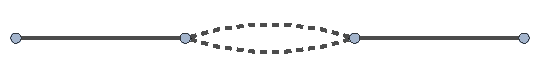
\includegraphics[width=0.6\linewidth]{img/0z92umyme84rx.pdf}
\end{figure}
\FloatBarrier

If you just want to plot the obtained graph, it is easier to process the
output of \texttt{FCLoopIntegralToGraph} directly with
\texttt{FCLoopGraphPlot}, which internally uses
\texttt{FCLoopAddEdgeTags}.

\begin{Shaded}
\begin{Highlighting}[]
\NormalTok{FCLoopIntegralToGraph}\OperatorTok{[}\NormalTok{FAD}\OperatorTok{[}\FunctionTok{p}\OperatorTok{,} \FunctionTok{p} \SpecialCharTok{{-}} \FunctionTok{k}\OperatorTok{],} \OperatorTok{\{}\FunctionTok{p}\OperatorTok{\}]} 
 
\NormalTok{FCLoopGraphPlot}\OperatorTok{[}\SpecialCharTok{\%}\OperatorTok{]}
\end{Highlighting}
\end{Shaded}

\begin{dmath*}\breakingcomma
\left\{\{-3\to 2,-1\to 1,1\to 2,1\to 2\},\{k,k,\{p,1,0\},\{p-k,1,0\}\},\left\{0,0,\frac{1}{(p^2+i \eta )},\frac{1}{((p-k)^2+i \eta )}\right\},1\right\}
\end{dmath*}

\FloatBarrier
\begin{figure}[!ht]
\centering
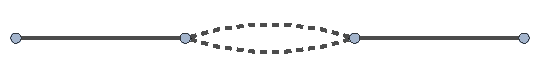
\includegraphics[width=0.6\linewidth]{img/18zlvfvc5dy6q.pdf}
\end{figure}
\FloatBarrier
\end{document}
